%%%%%%%%%%%%%%%%%%%%%%%%%%%%%%%%%%%%%%%%%
% a0poster Portrait Poster
% LaTeX Template
% Version 1.0 (22/06/13)
%
% The a0poster class was created by:
% Gerlinde Kettl and Matthias Weiser (tex@kettl.de)
% 
% This template has been downloaded from:
% http://www.LaTeXTemplates.com
%
% License:
% CC BY-NC-SA 3.0 (http://creativecommons.org/licenses/by-nc-sa/3.0/)
%
%%%%%%%%%%%%%%%%%%%%%%%%%%%%%%%%%%%%%%%%%

%----------------------------------------------------------------------------------------
%   PACKAGES AND OTHER DOCUMENT CONFIGURATIONS
%----------------------------------------------------------------------------------------

\documentclass[a0,portrait]{a0poster}

\usepackage{multicol} % This is so we can have multiple columns of text side-by-side
\columnsep=100pt % This is the amount of white space between the columns in the poster
\columnseprule=0pt % This is the thickness of the black line between the columns in the poster

\usepackage[svgnames]{xcolor} % Specify colors by their 'svgnames', for a full list of all colors available see here: http://www.latextemplates.com/svgnames-colors

\usepackage{times} % Use the times font
%\usepackage{palatino} % Uncomment to use the Palatino font

\usepackage{graphicx} % Required for including images
\graphicspath{{fig/}} % Location of the graphics files
\usepackage{booktabs} % Top and bottom rules for table
\usepackage[font=small,labelfont=bf]{caption} % Required for specifying captions to tables and figures
\usepackage{amsfonts, amsmath, amsthm, amssymb} % For math fonts, symbols and environments
\usepackage{wrapfig} % Allows wrapping text around tables and figures

\begin{document}

%----------------------------------------------------------------------------------------
%   POSTER HEADER 
%----------------------------------------------------------------------------------------

% The header is divided into two boxes:
% The first is 75% wide and houses the title, subtitle, names, university/organization and contact information
% The second is 25% wide and houses a logo for your university/organization or a photo of you
% The widths of these boxes can be easily edited to accommodate your content as you see fit
\begin{center}
{\veryHuge \color{NavyBlue} \textbf{Modelling of cardiac cross-bridge
cycling during ischemia}\\ [2cm]}% Title
\end{center}
%\Huge\textit{An Exploration of Complexity}\\[2cm] % Subtitle
\begin{minipage}[b]{0.63\linewidth}
\huge \textbf{Andrej Klic$\mathbf{^1}$, Mario
    Uhrin$\mathbf{^1}$ and Ivan Valent$\mathbf{^2}$}\\[0.4cm] % Author(s)
\Large $\mathbf{^1~}$Department of Physical Chemistry of Drugs, Faculty of Pharmacy\\
Comenius University, Bratislava, Slovakia \\[0.2cm]
\Large $\mathbf{^2~}$Department of Physical and Theoretical Chemistry, Faculty of Nat.~Sciences\\
Comenius University, Bratislava, Slovakia\\[0.2cm]
\Large Contact:~\texttt{andrej.klic@gmail.com}\\
\end{minipage}
%
\begin{minipage}[b]{0.45\linewidth}

\includegraphics[scale=0.45]{faf-prif_logos}\\
\end{minipage}

\vspace{1.3cm} % A bit of extra whitespace between the header and poster content

%----------------------------------------------------------------------------------------

\begin{multicols}{2} % This is how many columns your poster will be broken into, a portrait poster is generally split into 2 columns

%----------------------------------------------------------------------------------------
%   INTRODUCTION
%----------------------------------------------------------------------------------------

\color{SaddleBrown} % SaddleBrown color for the introduction

\section*{Introduction}

Metabolic changes caused by sudden oxygen delivery cutt-off are followed
by accumulation of specific metabolites affecting force of heart muscle
contraction. To closely evaluate those effects, we~modified and extended
the cardiac myo\-filament model proposed by Rice [1]. The presented
results of sensitivity analysis identified parameters with significant
impact on contractile force during ischemia.
%----------------------------------------------------------------------------------------
%THEORY
%----------------------------------------------------------------------------------------

\color{DarkSlateGray} % DarkSlateGray color for the rest of the content

\section*{Theory}

The key players in heart muscle contraction cycle are the two proteins,
the thin (actin) and thick (myosin) filaments, together with
Ca${^\mathrm{2+}}$ and ATP. 

The launch of the cycle depends on concentration of Ca${^\mathrm{2+}}$
in intracellular space. Action potential triggers massive elevation of
Ca${^\mathrm{2+}}$ in cell, which causes change of conformation of 
actin, enabling its contact with myosin. The influx of Ca${^\mathrm{2+}}$
thus results in connection of actin and myosin and forming the cross-bridge.

During ischemia, the accumulation of  H${\mathrm{^+}}$ and phosphates
occurs. The H${\mathrm{^+}}$ is binding on the neck of myosin head,
altering its conformation, resulting in weakening of the power-stroke.
Phosphate, if~present in hight concentration, is rebinding on myosin
head, thus preventing the formation of strong bound between actin and
myosin.

\begin{center}\vspace{0.8cm}
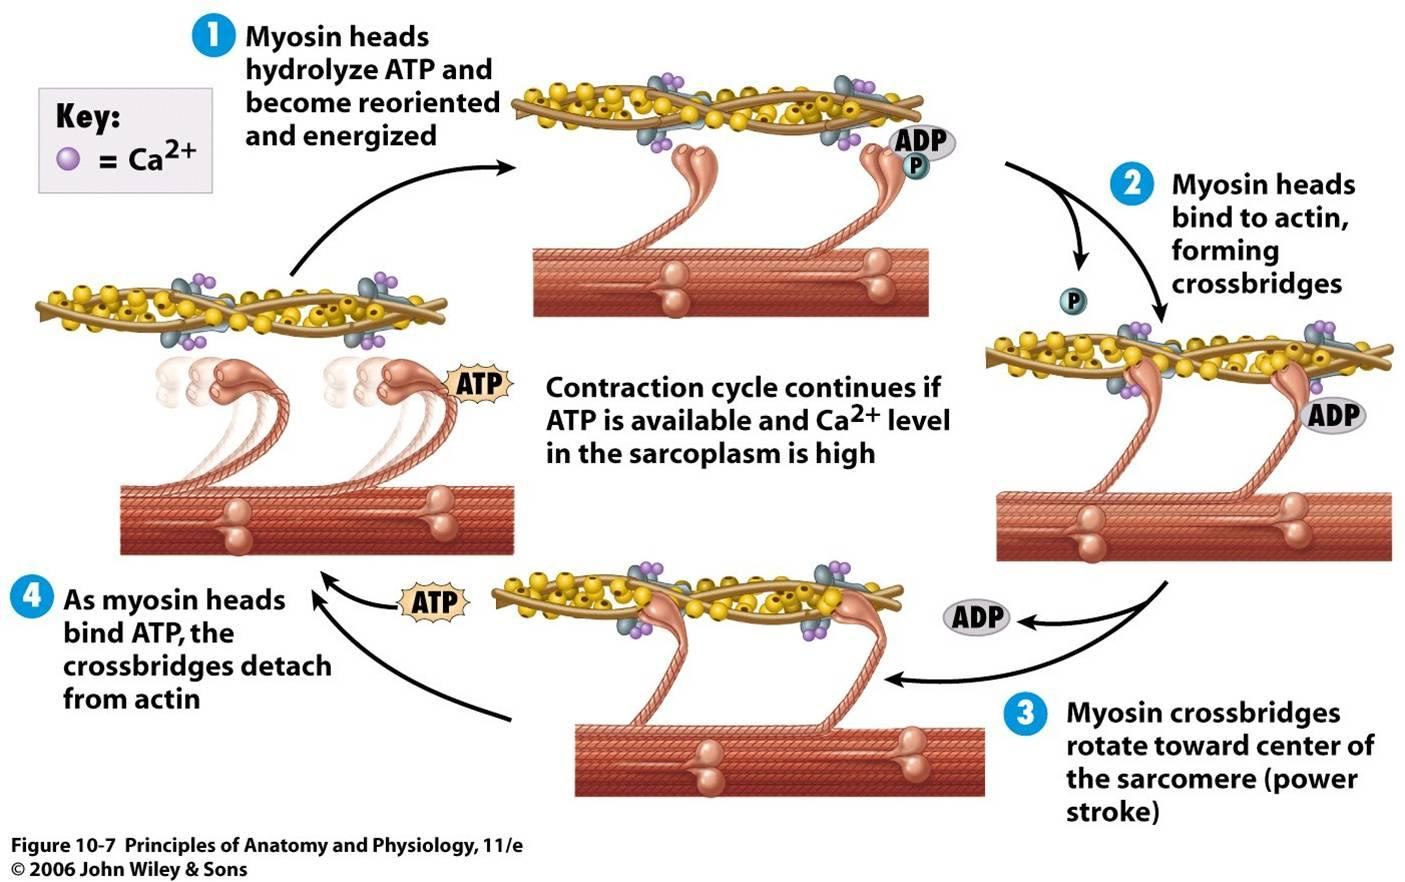
\includegraphics[scale=0.65]{muscle-contraction_hi-res}
\captionof{figure}{\color{DarkSlateGray} Physiology of the cross-bridge cycling. (Figure
reproduced, with generous consent of copyright holder, for educational and
noncommercial use only).}
\end{center}%\vspace{1cm}

%----------------------------------------------------------------------------------------
%   Implementation
%----------------------------------------------------------------------------------------

\section*{Implementation}

Mechanistic behavior of contraction cycle can be well captured into
mathematical model. The scheme below illustrates four underlying states
of cross-bridge cycle model. 

States N$_{\mathrm{XB}}$ and P$_{\mathrm{XB}}$ represent nonpermissive and
permissive conformations of the regulatory proteins, respectively. The
next transition is to the XB$_{\mathrm{PreR}}$ state, short for
prerotated, that is strongly bound with the myosin head extended. The
transition to the post-rotated force-generating state in dotted ellipse,
represents the isomerization inducing strain in the extensible myosin
head's neck region. The AM1 and AM2 are two strongly-bound
rapid-equilibrium states, where the virtual power-stroke occurs. After the
powerstroke, the ATP binds on myosin head, leading to disconection of
cross-bridge and shift of cycle to P$_{\mathrm{XB}}$ state.

\begin{center}%\vspace{1cm}
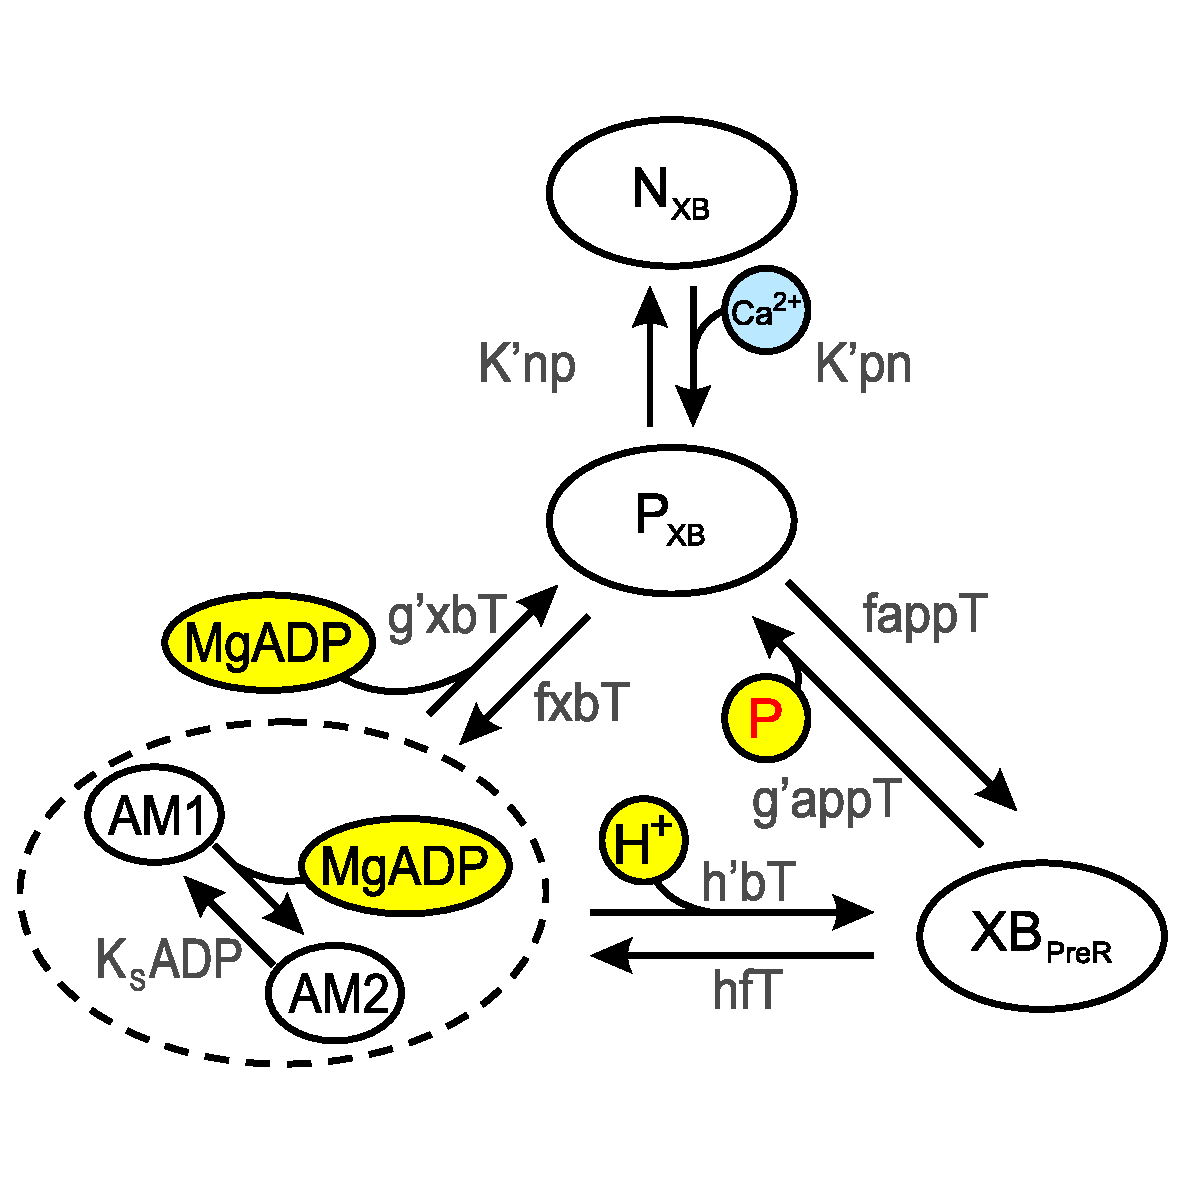
\includegraphics[scale=0.95]{cross-bridge_scheme_v2}
\captionof{figure}{\color{DarkSlateGray} Model construction. Scheme redrawn and modified after Tran [2].}
\end{center}%\vspace{1cm}

%----------------------------------------------------------------------------------------
%   Methods
%----------------------------------------------------------------------------------------

\section*{Methods}

Basic model [2] in CellML was exported and further revised in
Python programming language. Our model is using the mean-field
approximations implemented as set of ODEs. Sensitivity analysis was
performed using VODE integrator with BDF method from the Python SciPy
package. Resulting data were visualised with the ggplot2 plotting system
supplied in R programming language distribution. 

Our workflow was greatly facilitated by endorsing IPython, a rich
architecture for interactive scientific computing.

\vfill
\columnbreak

%----------------------------------------------------------------------------------------
%   RESULTS 
%----------------------------------------------------------------------------------------

\section*{Results}

\begin{center}%\vspace{1cm}
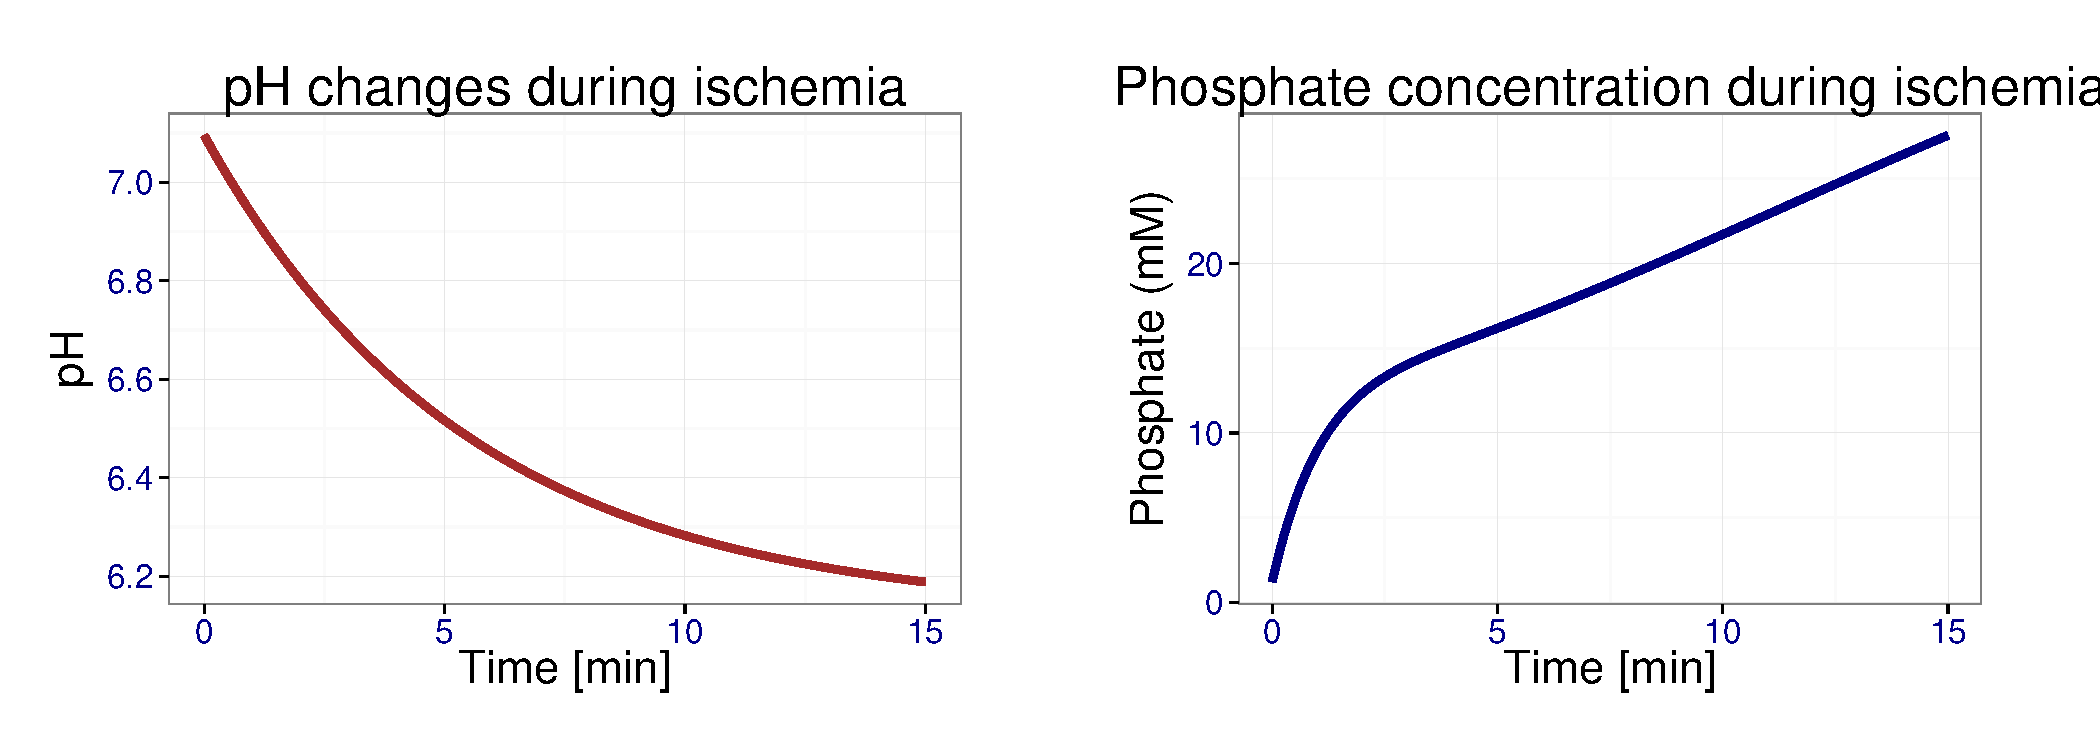
\includegraphics[scale=1.0]{fig/graf1}
\captionof{figure}{\color{DarkSlateGray} Simulation of ischemia. In sudden oxygen delivery cut-off, the
    metabolical changes occurs, which have direct impact on cycle of heart
    muscle contraction. The concentrations of ATP and creatine-phosphate are
    quickly decreasing and cumulation of ADP, phospates and protons occurs.
    The cell metabolism decreases and switches to anaerobic regime.}
\end{center}\vspace{1cm}

\begin{center}\vspace{1cm}
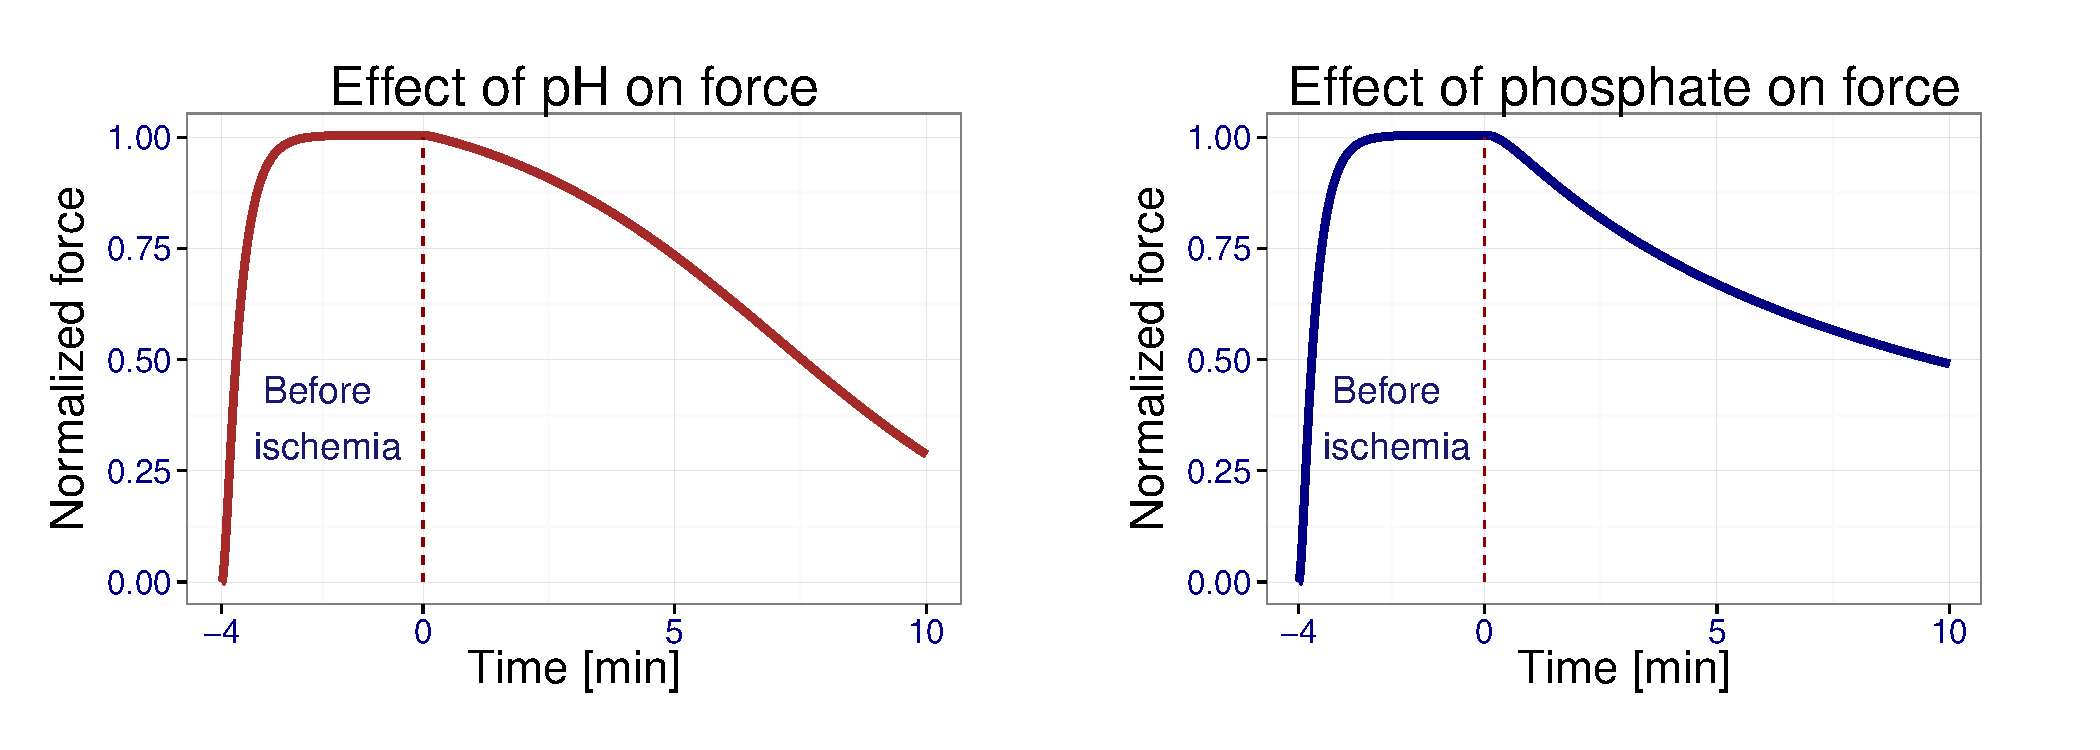
\includegraphics[scale=1.0]{fig/graf2}
\captionof{figure}{\color{DarkSlateGray} Effect of metabolites selected by sensitivity analysis
    on contraction force of cross-bridge. Build-up of protons and
    inorganic phosphate is characteristic for ischemia. These metabolites
    are directly interferring with phases of the cross-bridge cycle,
resulting in drop in contractile force of heart muscle.}
\end{center}\vspace{1cm}
    
    
\begin{center}\vspace{1cm}
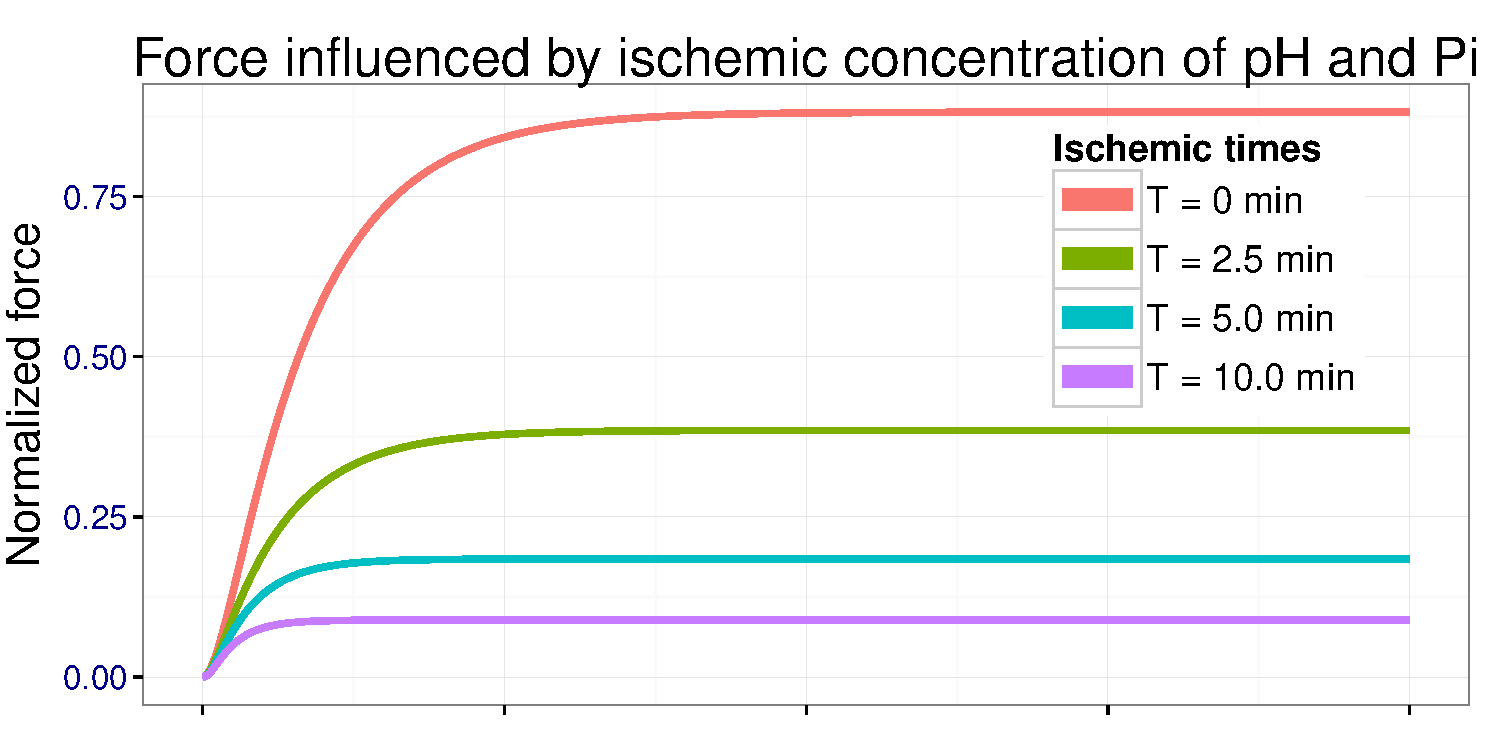
\includegraphics[scale=1.0]{fig/graf3}
\captionof{figure}{\color{DarkSlateGray} Influence on contractile force by ischemic
    concentrations of H${\mathrm{^+}}$ and P${\mathrm{_i}}$ in time.
    Concentration values are the same as in Fig.3. The concentration of
    H${\mathrm{^+}}$ and P${\mathrm{_i}}$ during every choosen timecourse
    remains constant during simulation.}
\end{center}\vspace{1cm}



%----------------------------------------------------------------------------------------
%   CONCLUSIONS
%----------------------------------------------------------------------------------------

\color{SaddleBrown} % SaddleBrown color for the conclusions to make them stand out

\section*{Conclusions}

\begin{itemize}

\item Sensitivity analysis identified the pH and phosphate as 
    strongest factors participating on decrease of contractile force

\item The 90\% drop in contractile force observed after 10 minutes of simulated
    ischemia correlates with in vivo experimental data obtained by
    Telkirdsen [3]

\end{itemize}


%----------------------------------------------------------------------------------------
%   FORTHCOMING RESEARCH
%----------------------------------------------------------------------------------------
\color{DarkSlateGray} % Set the color back to DarkSlateGray for the rest of the content

\section*{Forthcoming Research}

The follow-up research will be focused on extending the model with new
parameters relating with mitochondrial dysfunction. Such pathologic
conditions are related with hypoxia and subtler changes of metabolites in
time. Aditionally, we are planning to adapt the Ca${^\mathrm{2+}}$
regulation facilitated by ion channels and ryanodine receptors into our
model.

 %----------------------------------------------------------------------------------------
%   REFERENCES
%----------------------------------------------------------------------------------------
\section*{References}

J. J. Rice, F. Wang, D. M. Bers, and P. de Tombe. \textit{Biophys J.}, \textbf{95(5):}2368-2390, 2008.\\
K. Tran, N. P. Smith, D. S. Loiselle, and E. J. Crampin. \textit{Biophys J.}, \textbf{98(2):}267-376, 2010.\\
J. R. Terkildsen, et all. \textit{Am J Physiol Heart Circ Physiol}, \textbf{293(5):}H3036-H3045, 2007.

%\nocite{*} % Print all references regardless of whether they were cited in the poster or not
%\bibliographystyle{science} % Plain referencing style
%\bibliography{Heraeus_poster} % Use the example bibliography file sample.bib

%----------------------------------------------------------------------------------------
%   ACKNOWLEDGEMENTS
%----------------------------------------------------------------------------------------

\subsection*{Acknowledgements}

\small{Typesetting by {\LaTeX} using the \texttt{a0poster} class
created by Gerlinde~Kettl and Matthias~Weiser (\texttt{tex@kettl.de}).\\
Template downloadable from: \texttt{http://www.LaTeXTemplates.com} (License: CC BY-NC-SA 3.0)}

%----------------------------------------------------------------------------------------

\end{multicols}
\end{document}
